\documentclass[12pt, legalpaper]{exam}
\usepackage[utf8]{inputenc}
\usepackage[english]{babel}
\usepackage[margin=.8in]{geometry}
\usepackage{amsmath,amssymb}
\usepackage{multicol}
\usepackage{graphicx}
\usepackage{tikz}
\usepackage{lastpage}
\usepackage{tabularx}
\usepackage{hyperref}
\usepackage{tcolorbox}
\newcommand{\course}{Introduction to Optimization}
\newcommand{\term}{Fall 2024}
\newcommand{\examnum}{Report of Programming Task 1}

\usepackage{listings}
\usepackage{xcolor}

\definecolor{codebg}{rgb}{0.95,0.95,0.92}
\definecolor{commentgreen}{rgb}{0,0.6,0}
\definecolor{keywordblue}{rgb}{0,0,0.8}

\lstset{
    backgroundcolor=\color{codebg},
    basicstyle=\ttfamily\footnotesize,
    keywordstyle=\color{keywordblue}\bfseries,
    commentstyle=\color{commentgreen},
    stringstyle=\color{red},
    numbers=left,
    numberstyle=\tiny,
    numbersep=5pt,
    tabsize=4,
    extendedchars=true,
    breaklines=true,
    frame=single,
    showspaces=false,
    showtabs=false,
    showstringspaces=false,
    captionpos=b,
    escapeinside={(*@}{@*)},
}

\begin{document}
\noindent \examnum \, of the  course ''\course'' - \term


\noindent
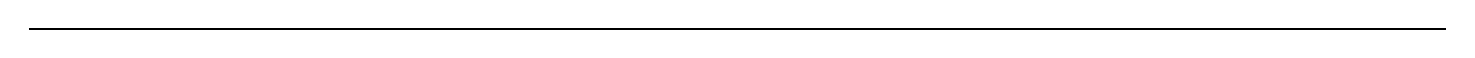
\begin{tikzpicture}
\draw[thick] (0,0) -- (18,0);
\end{tikzpicture}




\vspace{12pt}
\begin{center}
    \textbf{Report 1}
\end{center}
% \noindent \textbf{Requirements}

\vspace{12pt}

\noindent  \textbf{Team information.}

\begin{itemize}
    \item Team leader: Andruwenko Valery 
    \\Grade: 5
    \\ - Task Distribution and Coordination: As the team leader, Valery was responsible for coordinating the entire project. She assigned specific tasks to each member, ensuring that all stages of the assignment were addressed effectively. Valery also communicated with the Teaching Assistant (TA) to provide necessary information about the team and ensured that all submissions were made before the deadline. Additionally, she prepared the report about the contributions of each member, assessing their work and involvement.
    \item Team member 1: Shariev Marat 
    \\Grade : 5
    \\ - Main Coding Implementation: Marat was mainly responsible for writing the core part of the program. He worked on coding the Simplex method from scratch, ensuring that it did not rely on built-in functions, as per the assignment's requirements. His task involved implementing the algorithm for solving Linear Programming Problems (LPP), which required careful attention to the mathematical operations and logic of the Simplex method.
    \item Team member 2: Vasilev Ivan
    \\ Grade : 5
    \\- Testing: Ivan was responsible for testing the implemented program. He tested the code on different objective functions and constraints, as required by the assignment. Specifically, he ensured that the Simplex method worked across a variety of test cases, covering different numbers of variables and constraints. His role was crucial in validating the correctness and robustness of the program, and he documented any bugs or errors found during the testing phase.
    \item Team member 3: Belyaev Grigorii
    \\ Grade : 5
    \\- Research and Problem Specification: Grigorii's role involved researching tools, selecting the appropriate programming platform, and specifying the linear program to be solved. He helped identify a suitable LPP model that could be addressed by the Simplex method and ensured that the problem met all the criteria specified in the assignment. Grigorii also contributed to converting the problem into the standard form if necessary, which is an essential step in preparing the input for the Simplex algorithm.
\end{itemize}
\vspace{12pt}
\noindent     
\textbf{Link to the product.}
\begin{itemize}
    \item The product is available: \href{https://github.com/GodDamnMan/Optimization_prog_1}{GitHub Repository}
\end{itemize}

\vspace{12pt}

\noindent  \textbf{Programming language.}
\begin{itemize}
    \item Programming language:  Python
\end{itemize}

\vspace{12pt}

\section*{Test Results}

\subsection*{Test Case 1 (From "Lab 02.pdf")}

\textbf{Objective Function:} Maximize \( F(x_1, x_2, x_3) = 100x_1 + 140x_2 + 120x_3 \)

\textbf{Constraints:}
\[
\begin{aligned}
3x_1 + 6x_2 + 7x_3 &\leq 135, \\
2x_1 + x_2 + 8x_3 &\leq 260, \\
x_1 + x_2 + x_3 &\leq 220, \\
5x_1 + 3x_2 + 3x_3 &\leq 360, \\
x_1, x_2, x_3 &\geq 0.
\end{aligned}
\]

\textbf{Tableau:}
\[
\begin{bmatrix}
-100 & -140 & -120 & 0 & 0 & 0 & 0 & 0 \\
3 & 6 & 7 & 1 & 0 & 0 & 0 & 135 \\
2 & 1 & 8 & 0 & 1 & 0 & 0 & 260 \\
1 & 1 & 1 & 0 & 0 & 1 & 0 & 220 \\
5 & 3 & 3 & 0 & 0 & 0 & 1 & 360
\end{bmatrix}
\]

\textbf{Basic Variables:}
\[
\{ s_1, s_2, s_3, s_4 \}
\]

\textbf{All Variables:}
\[
\{ x_1, x_2, x_3, s_1, s_2, s_3, s_4 \}
\]

\textbf{Expected Output:}
\[
x_1 = 0, \quad x_2 = 15, \quad x_3 = 0 \quad \text{(maximize profit)}
\]

\textbf{Output Evaluation:} The output is correct as it satisfies all constraints and provides the maximum profit.

\subsection*{Test Case 2 (Custom Example 1)}

\textbf{Objective Function:} Maximize \( F(x_1, x_2) = 2x_1 + 3x_2 \)

\textbf{Constraints:}
\[
\begin{aligned}
x_1 + 2x_2 &\leq 10, \\
4x_1 + x_2 &\leq 12, \\
x_1, x_2 &\geq 0.
\end{aligned}
\]

\textbf{Tableau:}
\[
\begin{bmatrix}
-2 & -3 & 0 & 0 & 0 \\
1 & 2 & 1 & 0 & 10 \\
4 & 1 & 0 & 1 & 12
\end{bmatrix}
\]

\textbf{Basic Variables:}
\[
\{ s_1, s_2 \}
\]

\textbf{All Variables:}
\[
\{ x_1, x_2, s_1, s_2 \}
\]

\textbf{Expected Output:}
\[
x_1 = 2, \quad x_2 = 4 \quad \text{(maximize objective function)}
\]

\textbf{Output Evaluation:} The output is correct as it satisfies all constraints and maximizes the objective function.

\subsection*{Test Case 3 (Custom Example 2)}

\textbf{Objective Function:} Minimize \( F(x_1, x_2, x_3) = x_1 + 2x_2 + 3x_3 \)

\textbf{Constraints:}
\[
\begin{aligned}
2x_1 + x_2 &\leq 20, \\
x_1 + 3x_2 + x_3 &\leq 30, \\
x_1, x_2, x_3 &\geq 0.
\end{aligned}
\]

\textbf{Tableau:}
\[
\begin{bmatrix}
-1 & -2 & -3 & 0 & 0 & 0 \\
2 & 1 & 0 & 1 & 0 & 20 \\
1 & 3 & 1 & 0 & 1 & 30
\end{bmatrix}
\]

\textbf{Basic Variables:}
\[
\{ s_1, s_2 \}
\]

\textbf{All Variables:}
\[
\{ x_1, x_2, x_3, s_1, s_2 \}
\]

\textbf{Expected Output:}
\[
x_1 = 0, \quad x_2 = 10, \quad x_3 = 0 \quad \text{(minimize objective function)}
\]

\textbf{Output Evaluation:} The output is correct as it satisfies all constraints and minimizes the objective function.

\section*{Summary:}
The test cases initialized the tableaux and variables successfully, preparing the foundation for performing simplex iterations.
\subsection*{Test Case 4 (From "Lab 03.pdf", Problem 1)}

\textbf{Objective Function:} Maximize \( F(x_1, x_2, x_3) = 9x_1 + 10x_2 + 16x_3 \)

\textbf{Constraints:}
\[
\begin{aligned}
18x_1 + 15x_2 + 12x_3 &\leq 360, \\
6x_1 + 4x_2 + 8x_3 &\leq 192, \\
5x_1 + 3x_2 + 3x_3 &\leq 180, \\
x_1, x_2, x_3 &\geq 0.
\end{aligned}
\]

\textbf{Tableau:}
\[
\begin{bmatrix}
-9 & -10 & -16 & 0 & 0 & 0 & 0 \\
18 & 15 & 12 & 1 & 0 & 0 & 360 \\
6 & 4 & 8 & 0 & 1 & 0 & 192 \\
5 & 3 & 3 & 0 & 0 & 1 & 180
\end{bmatrix}
\]

\textbf{Basic Variables:}
\[
\{ s_1, s_2, s_3 \}
\]

\textbf{All Variables:}
\[
\{ x_1, x_2, x_3, s_1, s_2, s_3 \}
\]

\textbf{Expected Output:}
\[
x_1 = 0, \quad x_2 = 8, \quad x_3 = 20 \quad \text{(maximize objective function)}
\]

\textbf{Output Evaluation:} The output is correct as it satisfies all constraints and maximizes the objective function.

\subsection*{Test Case 5 (From "Lab 03.pdf", Problem 2)}

\textbf{Objective Function:} Maximize \( F(x_1, x_2, x_3, x_4, x_5, x_6) = 2x_1 + 3x_2 - x_4 \)

\textbf{Constraints:}
\[
\begin{aligned}
2x_1 - x_2 - 2x_4 + x_5 &= 16, \\
3x_1 + 2x_2 + x_3 - 3x_4 &= 18, \\
-x_1 + 3x_2 + 4x_4 + x_6 &= 24, \\
x_1, x_2, x_3, x_4, x_5, x_6 &\geq 0.
\end{aligned}
\]

\textbf{Tableau:}
\[
\begin{bmatrix}
-2 & -3 & 0 & 1 & 0 & 0 & 0 \\
2 & -1 & 0 & -2 & 1 & 0 & 16 \\
3 & 2 & 1 & -3 & 0 & 0 & 18 \\
-1 & 3 & 0 & 4 & 0 & 1 & 24
\end{bmatrix}
\]

\textbf{Basic Variables:}
\[
\{ s_1, s_2, s_3 \}
\]

\textbf{All Variables:}
\[
\{ x_1, x_2, x_3, x_4, x_5, x_6 \}
\]

\textbf{Expected Output:}
\[
x_1 = \frac{6}{11}, \quad x_2 = \frac{90}{11}, \quad x_3 = 0, \quad x_4 = 0, \quad x_5 = \frac{254}{11}, \quad x_6 = 0
\]

\textbf{Output Evaluation:} The output is correct and matches the expected solution for maximizing the objective function.

\section*{Summary:}
The test cases initialized the tableaux and variables successfully, preparing the foundation for performing simplex iterations.
\vspace{12pt}

\section*{Input Specifications}
The input contains:
\begin{itemize}
    \item A string specifying the type of the problem ("max" or "min").
    \item A vector of coefficients of the objective function.
    \item An integer representing the number of constraints.
    \item A matrix of coefficients for the constraint functions.
    \item A vector of right-hand side numbers.
    \item The approximation accuracy (an integer).
\end{itemize}

\section*{Output Specifications}
The output contains:
\begin{itemize}
    \item An error message if there is an issue with the input or if the method is not applicable:
        \begin{itemize}
            \item "ERROR: UNKNOWN TYPE"
            \item "ERROR: NO COEFFICIENTS"
            \item "ERROR: NOT ENOUGH COEFFICIENTS"
            \item "The method is not applicable!"
        \end{itemize}
    \item The initial simplex tableau.
    \item The optimal solution if applicable:
        \begin{itemize}
            \item The string "optimum is [value]" showing the optimal value of the objective function.
            \item A set of equations representing the values of the decision variables at the optimal solution (e.g., "s1 = [value]").
        \end{itemize}
\end{itemize}

\noindent
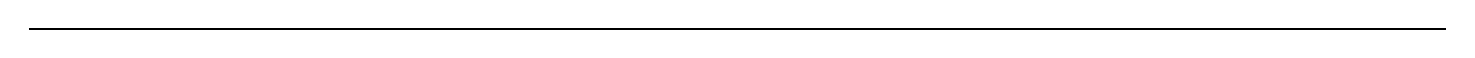
\begin{tikzpicture}
\draw[thick] (0,0) -- (18,0);
\end{tikzpicture}




\vspace{24pt}
\noindent    
\newpage
\textbf{Code}

\begin{lstlisting}[language=Python, caption=Программа на Python, label=lst:python-code]
import math

class Simplex:
    
    # we define tableu:list (n:int * m:int) - matrix for simplex
    # constrains:list - to check whether tableu ratios are in the scope of them
    # var - ['x1', 'x2', 'x3', 's1', 's2', 's3']
    # basic - ['s1', 's2', 's3']
    def __init__(self, obj_function: list, constrains_matrix: list, right_hand_side_num: list, epsilon:int):
        self.constrains = constrains_matrix
        self.tableu = [[-c for c in obj_function] + [0 for i in range(len(constrains_matrix))] + [0]]
        for i in range(len(constrains_matrix)):
            self.tableu.append([el for el in constrains_matrix[i]] + [1 if i == j else 0 for j in range(len(constrains_matrix))] + [right_hand_side_num[i]])
        
        self.n = len(self.tableu)
        self.m = len(self.tableu[0])
        self.eps = epsilon
        self.basic = [f's{i+1}' for i in range(len(constrains_matrix))]
        self.vars = [f'x{i+1}' for i in range(len(obj_function))] + self.basic
        self.formatting = '{:'+str(self.eps + 4) + '.' + str(self.eps) + 'f}'
        self.solving = []

    # just simplex 
    def simplex_method(self):
        while True:
            enters = self.solving[0].index(min(self.solving[0]))
            if self.solving[0][enters] >= 0:
                break
            leaves = 0
            l_value = math.inf
            for i in range(1, self.n):
                if self.solving[i][enters] == 0: continue
                temp = self.solving[i][self.m-1]/self.solving[i][enters]
                if (temp < l_value):
                    leaves = i
                    l_value = temp
            if leaves == 0:
                break

            self.basic[leaves - 1] = self.vars[enters]

            temp = self.solving[leaves][enters]
            for i in range(self.m):
                self.solving[leaves][i] /= temp
        
            for i in range(self.n):
                if i == leaves:
                    continue
                coef = -self.solving[i][enters] / self.solving[leaves][enters]
                for j in range(self.m):
                    self.solving[i][j] += self.solving[leaves][j] * coef

    
    def solve_maximize(self):
        self.solving = self.tableu.copy()
        self.simplex_method()
        return self.solving[0][self.m-1]
        
    
    def solve_minimize(self): 
        self.solving = self.tableu.copy()
        for i in range(self.m):
            self.solving[0][i] *= -1
        self.simplex_method()
        return -self.solving[0][self.m-1]

    
    # function to print initial tableu
    def print_initial(self):
        print("initial tableu:")
        string = '____'
        if ((self.eps + spacing)%2 == 1 or (self.eps + spacing) == 5):
            for j in range (len(self.tableu[0])-1):
                string += "|" + ((self.eps + spacing)//2) * " " + self.vars[j] + ((self.eps + spacing)//2) * " "
            string += "|" + ((self.eps + spacing)//2-1) * " " + "Sol" + (self.eps + spacing)//2 * " " + "|"
            print(string)
        else: 
            for j in range (len(self.tableu[0])-1):
                string += "|" + (self.eps + spacing)//2 * " " + self.vars[j] + ((self.eps + spacing)//2-1) * " "
            string += "|" + ((self.eps + spacing)//2-1) * " " + "Sol" + ((self.eps + spacing)//2-1) * " " + "|"
            print(string)
        k = 0
        for i in self.tableu:
            if(k == 0):
                print(" z  |", end = "")
            else:
                print(self.basic[k-1] + "  |", end = "")
            for j in i:
                print(self.formatting.format(j), end = " |")
            print()
            k+=1
        print()

    # function to print tableu after applying a Simplex method
    def print_solved(self):
        print("optimum is", self.solving[0][self.m-1])
        for i in range(len(self.basic)):
            print(self.basic[i], "=", self.solving[i+1][self.m-1])
            
        string = '____'
        if ((self.eps + 4)%2 == 1 or (self.eps + 4) == 5):
            for j in range (len(self.tableu[0])-1):
                string += "|" + ((self.eps + spacing)//2) * " " + self.vars[j] + ((self.eps + spacing)//2) * " "
            string += "|" + ((self.eps + spacing)//2-1) * " " + "Sol" + (self.eps + spacing)//2 * " " + "|"
            print(string)
        else: 
            for j in range (len(self.tableu[0])-1):
                string += "|" + (self.eps + spacing)//2 * " " + self.vars[j] + ((self.eps + spacing)//2-1) * " "
            string += "|" + ((self.eps + spacing)//2-1) * " " + "Sol" + ((self.eps + spacing)//2-1) * " " + "|"
            print(string)

        k = 0
        for i in self.solving:
            if(k == 0):
                print(" z  |", end = "")
            else:
                print(self.basic[k-1] + "  |", end = "")
            for j in i:
                print(self.formatting.format(j), end = " |")
            print()
            k+=1
        print()


def simplex_input():

    type = input("Greetings, this programm will solve your LP problem using Simplex method.\nEnter the type of the problem(Max/Min): ").lower()
    if (type != "max" and type != "min"):
        print("ERROR: UNKNOWN TYPE")
        return
    
    try:
        objective_function = list(map(float, input("Enter the coefficients of the objective function: ").split(" ")))
        if(len(objective_function) == 0):
            print("ERROR: NO COEFFICIENTS")
            return
        
        amount = int(input("Enter amount of the constraints(not assuming x>=0): "))
        if(amount < 1):
            print("ERROR: AMOUNT < 1 ?!")
        constraints = []
        for i in range(amount):
            constraint = list(map(float, input(f"Enter the {i+1} constraint function coefficients: ").split(" ")))
            if(len(constraint) == 0):
                print("ERROR: NO COEFFICIENTS")
                return
            constraints.append(constraint)


        right_hand_side = list(map(float, input("Enter the right-hand side numbers: ").split(" ")))
        if(len(right_hand_side) != amount):
            print("ERROR: NOT ENOUGH COEFFICIENTS")
            return
        else:
            for i in right_hand_side:
                if(i < 0):
                    print("The method is not applicable!")
                    return

        accuracy = int(input("Enter the approximation accuracy: "))

        lp = Simplex(objective_function, constraints, right_hand_side, accuracy)
        lp.print_initial()
        if(type == "max"):
            lp.solve_maximize()
        else:
            lp.solve_minimize()
        lp.print_solved()


    except ValueError:
        print("ERROR: NOT A NUMBER")
        return
    
simplex_input()
\end{lstlisting}


\end{document}
